\documentclass[10pt,twocolumn]{article}
\usepackage[margin=0.68in,columnsep=0.24in]{geometry}
\usepackage[T1]{fontenc}
\usepackage[utf8]{inputenc}
\usepackage{lmodern}
\usepackage{microtype}
\usepackage{amsmath,amssymb,amsthm}
\usepackage{booktabs}
\usepackage{graphicx}
\usepackage{xcolor}
\usepackage{enumitem}
\usepackage{hyperref}

\hypersetup{
  colorlinks=true,
  linkcolor=blue!60!black,
  citecolor=blue!60!black,
  urlcolor=blue!60!black,
  pdftitle={Certified Verification of Improved Downward-Closed Delegation Bounds},
  pdfauthor={Lluis Eriksson}
}

\newtheorem{proposition}{Proposition}
\newcommand{\QQ}{\mathbb{Q}}
\newcommand{\ZZ}{\mathbb{Z}}
\newcommand{\NN}{\mathbb{N}}

\title{\vspace{-1.1em}\textbf{Certified Verification of Improved Downward-Closed Delegation Bounds}}
\author{Lluis Eriksson\thanks{Independent Researcher. Code, Lean~4 proofs, and certificates: MIT License; manuscript and figures: CC-BY-4.0. Prepared with AI coding, formalization, and drafting assistance from Google Antigravity; all proofs, exact-$\QQ$ verifiers, and adversarial tests were independently compiled and verified locally. Repository: \url{https://github.com/lluiseriksson/delegation-29-70-certificates}}}
\date{November 25, 2026}

\begin{document}
\maketitle
\vspace{-1.4em}

\begin{abstract}
Hamed Abdi, Kiarash Banihashem, MohammadTaghi Hajiaghayi, and Danny Mittal (\texttt{arXiv:2611.33095}, Nov.\ 2026) dramatically improved the universal approximation guarantee for agent-oblivious combinatorial delegation under downward-closed constraints from $0.1098$ to a deterministic menu achieving $> 29/70 \approx 0.41429$ (with a self-contained analytic $3/10$ warm-up), while separating downward-closed delegation strictly below the matroid optimum of $1/2$: a five-item knapsack caps deterministic menus at $500/1011$ and randomized rules at $5011/10110$ (asymptotically $30/61$), and a computer-assisted family caps all randomized rules below $9621/20000 = 0.48105$. We build a standalone zero-dependency \textbf{Lean~4.35.0} formalization of 18 core score, forced-item, Efron--Stein, Bernstein-polynomial, seed-reserve, and impossibility theorems (zero \texttt{sorry}, zero warnings, zero \texttt{Classical.choice}) paired with an exact-$\QQ$ four-mode certificate verifier (\texttt{DC-DELEG-CERT-1.0}). Across 16 canonical certificates ($0.185$--$2.611\,\mathrm{ms}$, total $9.21\,\mathrm{ms}$), all five-item knapsack bounds, Lemma~4.4 Bernstein positivity certificates, Algorithm~2 capped-menu scores, and Appendix~A alternating-Taylor $\beta < 0.48105$ brackets replay identically over $\QQ$ while rejecting 60/60 live adversarial forgery attacks.
\end{abstract}

\section{Introduction}\label{sec:intro}
In combinatorial delegated choice~\cite{holmstrom1984delegation,kleinberg2018delegated,banihashem2025delegated}, a principal commits to an acceptance rule over a downward-closed family $\mathcal{F} \subseteq 2^E$ without transfers, and an informed agent observing independent item pairs $(X_i, Y_i)$ ($X_i \ge 0, Y_i > 0$, arbitrarily correlated within each item) submits an acceptable feasible set maximizing $Y(S)$ (breaking ties against the principal). While matroids admit an optimal deterministic guarantee of $1/2$~\cite{bechtel2021delegated,abdi2026matroid} and downward-closed prophet inequalities admit no constant factor~\cite{rubinstein2016beyond}, Abdi et al.~\cite{abdi2026downward} established sharp new bounds $29/70 < \alpha_D \le \alpha_R < 0.48105$:
\begin{enumerate}[leftmargin=*,nosep]
  \item \textbf{Five-Item Knapsack Separation (Sec.~3):} A 5-item capacity-3 knapsack with offline optimum $V = 1011/50$ caps every deterministic menu at $10$ ($500/1011 < 1/2$, Prop.~3.1) and every randomized rule (even knowing agent utilities) at $5011/500$ ($5011/10110 < 1/2$ at $\eta = 1/100$, Thm.~3.2), lowering to $30/61$ as $\varepsilon, \eta \downarrow 0$ (Prop.~3.3).
  \item \textbf{Analytic $3/10$ Warm-Up \& Bernstein Certificate (Sec.~4):} A single total-value threshold achieves $B(z) = z\Pr[W \ge z] + e(z)\Pr[W < z]$ via forced items (Lem.~4.2), an Efron--Stein variance bound $\operatorname{Var}(Z_{3/2}) \le \frac{3}{2}\mu$~\cite{efron1981jackknife} (Lem.~4.3), and a scalar proof $\mu + a < 10/3$ (Lem.~4.4) anchored by a degree-7 Bernstein positivity certificate on $[2/13, 2/5]$ and $[2/5, 2/3]$.
  \item \textbf{Capped Menus, Seeds, \& $29/70$ Guarantee (Sec.~2, 5):} Score lower bounds $b_M(x)$ (Lem.~2.1), safe-singleton normalization (Lem.~2.2), and Algorithm~2 capped menus with seeds ($b_P = t + \min_{i\in P} w_i - w(P) > 0$) certify $> 29/70\,V$ (Thm.~5.1).
  \item \textbf{Randomized Ceiling $\beta < 0.48105$ (App.~A):} Alternating degree-18/19 Taylor brackets for $e^{-z}, e^{-b}$ with rational $a = 67/100, b = 9/200, d = 9/50, \Delta = 1/400$ certify $\beta \le 0.481043999746 < 9621/20000$.
\end{enumerate}

\paragraph{Contributions and Scope.}
We do not re-formalize continuous Harris--FKG integration, the 96-interval LP infeasibility solver of Sec.~10, or the 1024-cell Lagrangian DP of App.~A.3--A.4 inside Lean~4; instead, we machine-check every core algebraic, list-combinatorial, Bernstein, menu-score, and Taylor-bracket pillar of~\cite{abdi2026downward}:
(i)~18 zero-\texttt{sorry}, zero-\texttt{Classical.choice} \textbf{Lean~4.35.0}~\cite{demoura2021lean4} theorems in \texttt{DownwardDelegation.lean};
(ii)~the exact-$\QQ$ verifier \texttt{DC-DELEG-CERT-1.0};
(iii)~16 canonical certificates across all four modes; and
(iv)~a 60-attack live red-team suite with 40-artifact SHA-256 manifest enforcement.

\section{Constructive Lean~4.35.0 Kernel}\label{sec:lean}
The standalone module \texttt{lean/DownwardDelegation.lean} compiles cleanly under Lean~4.35.0 with zero external dependencies, zero warnings, and zero \texttt{sorry}. Auditing all 18 theorems via \texttt{\#print axioms} (\texttt{AuditAxioms.lean}) confirms 8 zero-axiom theorems (\texttt{none}), 10 using \texttt{[propext, Quot.sound]}, and \textbf{0} using \texttt{Classical.choice} or \texttt{Lean.ofReduceBool} (Table~\ref{tab:lean}).

\begin{table}[t]
\centering
\caption{All 18 machine-checked Lean~4.35.0 theorems in \texttt{DownwardDelegation.lean} (zero \texttt{sorry}, zero \texttt{Classical.choice}).}
\label{tab:lean}
\scriptsize
\setlength{\tabcolsep}{2.6pt}
\begin{tabular}{@{}rlll@{}}
\toprule
\# & Lean Theorem Identifier & Paper Ref. & Axioms \\
\midrule
1 & \texttt{universal\_bounds\_hierarchy} & Thm.~1.1--1.2 & \texttt{none} \\
2 & \texttt{knapsack5\_offline\_optimum\_exact} & Eq.~3.1 & \texttt{none} \\
3 & \texttt{knapsack5\_agent\_strict\_ranking} & Prop.~3.1 & \texttt{p, Q} \\
4 & \texttt{knapsack5\_det\_upper\_bound\_exact} & Prop.~3.1 & \texttt{none} \\
5 & \texttt{knapsack5\_rand\_case\_bounds} & Thm.~3.2 & \texttt{p, Q} \\
6 & \texttt{knapsack5\_rand\_asymptotic\_30\_61} & Prop.~3.3 & \texttt{p, Q} \\
7 & \texttt{menu\_score\_payoff\_bound} & Lem.~2.1 & \texttt{p, Q} \\
8 & \texttt{forced\_item\_pointwise\_decomposition} & Lem.~4.2 & \texttt{p, Q} \\
9 & \texttt{threshold\_tail\_bound\_monotone} & Eq.~4.3 & \texttt{p, Q} \\
10 & \texttt{efron\_stein\_step\_bound} & Lem.~4.3 & \texttt{p, Q} \\
11 & \texttt{cantelli\_mean\_cap\_lt\_5} & Lem.~4.4 & \texttt{p, Q} \\
12 & \texttt{lemma44\_case1\_gamma\_pos} & Lem.~4.4 & \texttt{none} \\
13 & \texttt{lemma44\_exp\_taylor7\_bound} & Eq.~4.11 & \texttt{none} \\
14 & \texttt{lemma44\_bernstein\_poly\_eval\_endpoints} & Lem.~4.4 & \texttt{none} \\
15 & \texttt{seed\_reserve\_margin\_positive} & Eq.~5.1--5.2 & \texttt{p, Q} \\
16 & \texttt{capped\_menu\_rescale\_equivariance} & Sec.~2.3, Alg.~2 & \texttt{p, Q} \\
17 & \texttt{main\_theorem\_ratio\_recip\_exact} & Sec.~2.3, 5.1 & \texttt{none} \\
18 & \texttt{appendix\_a\_beta\_strict\_bound} & App.~A.6.1 & \texttt{none} \\
\bottomrule
\end{tabular}
\vspace{-0.4em}
\begin{flushleft}
\tiny Axiom key: \texttt{none} = zero axioms (8); \texttt{p, Q} = \texttt{[propext, Quot.sound]} (10).
\end{flushleft}
\vspace{-0.8em}
\end{table}

\begin{proposition}[Machine-Checked Core Identities]\label{prop:lean}
The Lean~4.35.0 kernel establishes the following universal identities over $\ZZ$ and arbitrary finite lists:
\begin{enumerate}[leftmargin=*,nosep]
  \item \emph{Inductive List Lemmas (Thms.~7, 8, 10, 15, 16):} For any nonempty accepted-value list $a::\mathrm{rest}$, $\mathrm{listMinNE}\,a\,\mathrm{rest} \le s$ for all $s \in a::\mathrm{rest}$; any nonnegative list with $\sum w_i \ge z$ obeys $\sum \min(w_i, z) \ge z$; any list with $0 \le \Delta_i \le c$ satisfies $\sum \Delta_i^2 \le c\sum \Delta_i$; any seed list satisfies $b_P = t + \min w_i - \sum w_i > 0$; and clipping/summing commutes with any positive scale $\lambda > 0$.
  \item \emph{Impossibility \& Analytic Bounds (Thms.~1--6, 11--14, 17--18):} Exact cleared arithmetic certifies $0.1098 < 3/10 < 29/70 < 0.48105 < 30/61 < 500/1011 < 5011/10110 < 1/2$, $V = 1011/50$, $10 + \frac{77}{50}\eta \le 10 + \frac{11}{5}\eta$, Cantelli contradiction $22\mu^2 \ge 25s(2\mu+12s)$ for $\mu \ge 5s$, Case~1 lower bound $168034/70785 > 0$, degree-7 Taylor gap $3772963/234881024 > 0$, and $P(b) > 0$ at knots $\{2/13, 2/5, 2/3\}$.
\end{enumerate}
\end{proposition}

\section{Exact-\texorpdfstring{$\QQ$}{Q} Verifier}\label{sec:cert}
The verifier \texttt{DC-DELEG-CERT-1.0} (\texttt{src/delegation\_certifier.py}, \texttt{src/delegation\_exact.py}) uses Python \texttt{fractions.Fraction} exclusively (source-audited for zero \texttt{float(}, \texttt{math.}, or \texttt{numpy}). Every payload enforces strict JSON typing, nesting-depth cap $32$, anchored canonical rational parsing (\texttt{\textbackslash A...\textbackslash Z}, forbidding \texttt{"-0"}, reduced denominators $\ge 2$, 2048-bit caps), and exact key sets across four modes:
\begin{enumerate}[leftmargin=*,nosep]
  \item \textbf{Mode~1 (Sec.~3 Five-Item Knapsack):} Enumerates all $2^5$ subsets, checks downward closure and strict agent ranking $C \succ AE \succ AB \succ E \succ A \succ B \succ J$, computes exact offline optimum $V$, $r_{ab}$ table, deterministic ratio $10/V < 1/2$, and Theorem~3.2/Prop.~3.3 randomized Case~1--2 bounds.
  \item \textbf{Mode~2 (Sec.~4 Lemma~4.4 Bernstein $3/10$):} Independently expands $P(\ell + (r-\ell)v)$ in $\QQ[v]$, computes all 8 degree-7 Bernstein coefficients $\beta_k = \sum_{j=0}^k \frac{\binom{k}{j}}{\binom{7}{j}} p_j > 0$, and replays the Cantelli, Case~1 ($168034/70785$), and degree-7 Taylor ($\ln(13/2) < 15/8$) bounds.
  \item \textbf{Mode~3 (Sec.~2, 5 Alg.~2 Capped Menu Scores):} Verifies downward closure, executes exact Algorithm~2 acceptance across all three body types (\texttt{total\_threshold}, \texttt{seeds\_upper}, \texttt{seeds\_reserve}) over all joint realizations, checks Lemma~2.2 safe-singleton normalization, seed reserve $b_P > 0$, and exact expected score $\mathbb{E}[b_M(X)]/V$.
  \item \textbf{Mode~4 (App.~A.5--A.6 Alternating-Taylor $\beta$):} Computes exact alternating Taylor brackets for $e^{-(a+b)}$ and $e^{-b}$, checks $v_{\mathrm{lo}} + \Delta - 1 > b$ and Eq.~(A.18) bracket positivity, and certifies exact 12-decimal brackets $[\beta_{\mathrm{lo}}, \beta_{\mathrm{hi}}]$ strictly below $9621/20000 = 0.48105$.
\end{enumerate}

\section{Empirical Atlas and Red-Team Audit}\label{sec:results}
Running \texttt{run\_all\_experiments.py} generates 16 canonical certificates (4 per mode) and four exact-$\QQ$ datasets, audited end-to-end by \texttt{verify\_all.py} with SHA-256 verification across all 40 tracked artifacts.

\begin{figure}[t]
  \centering
  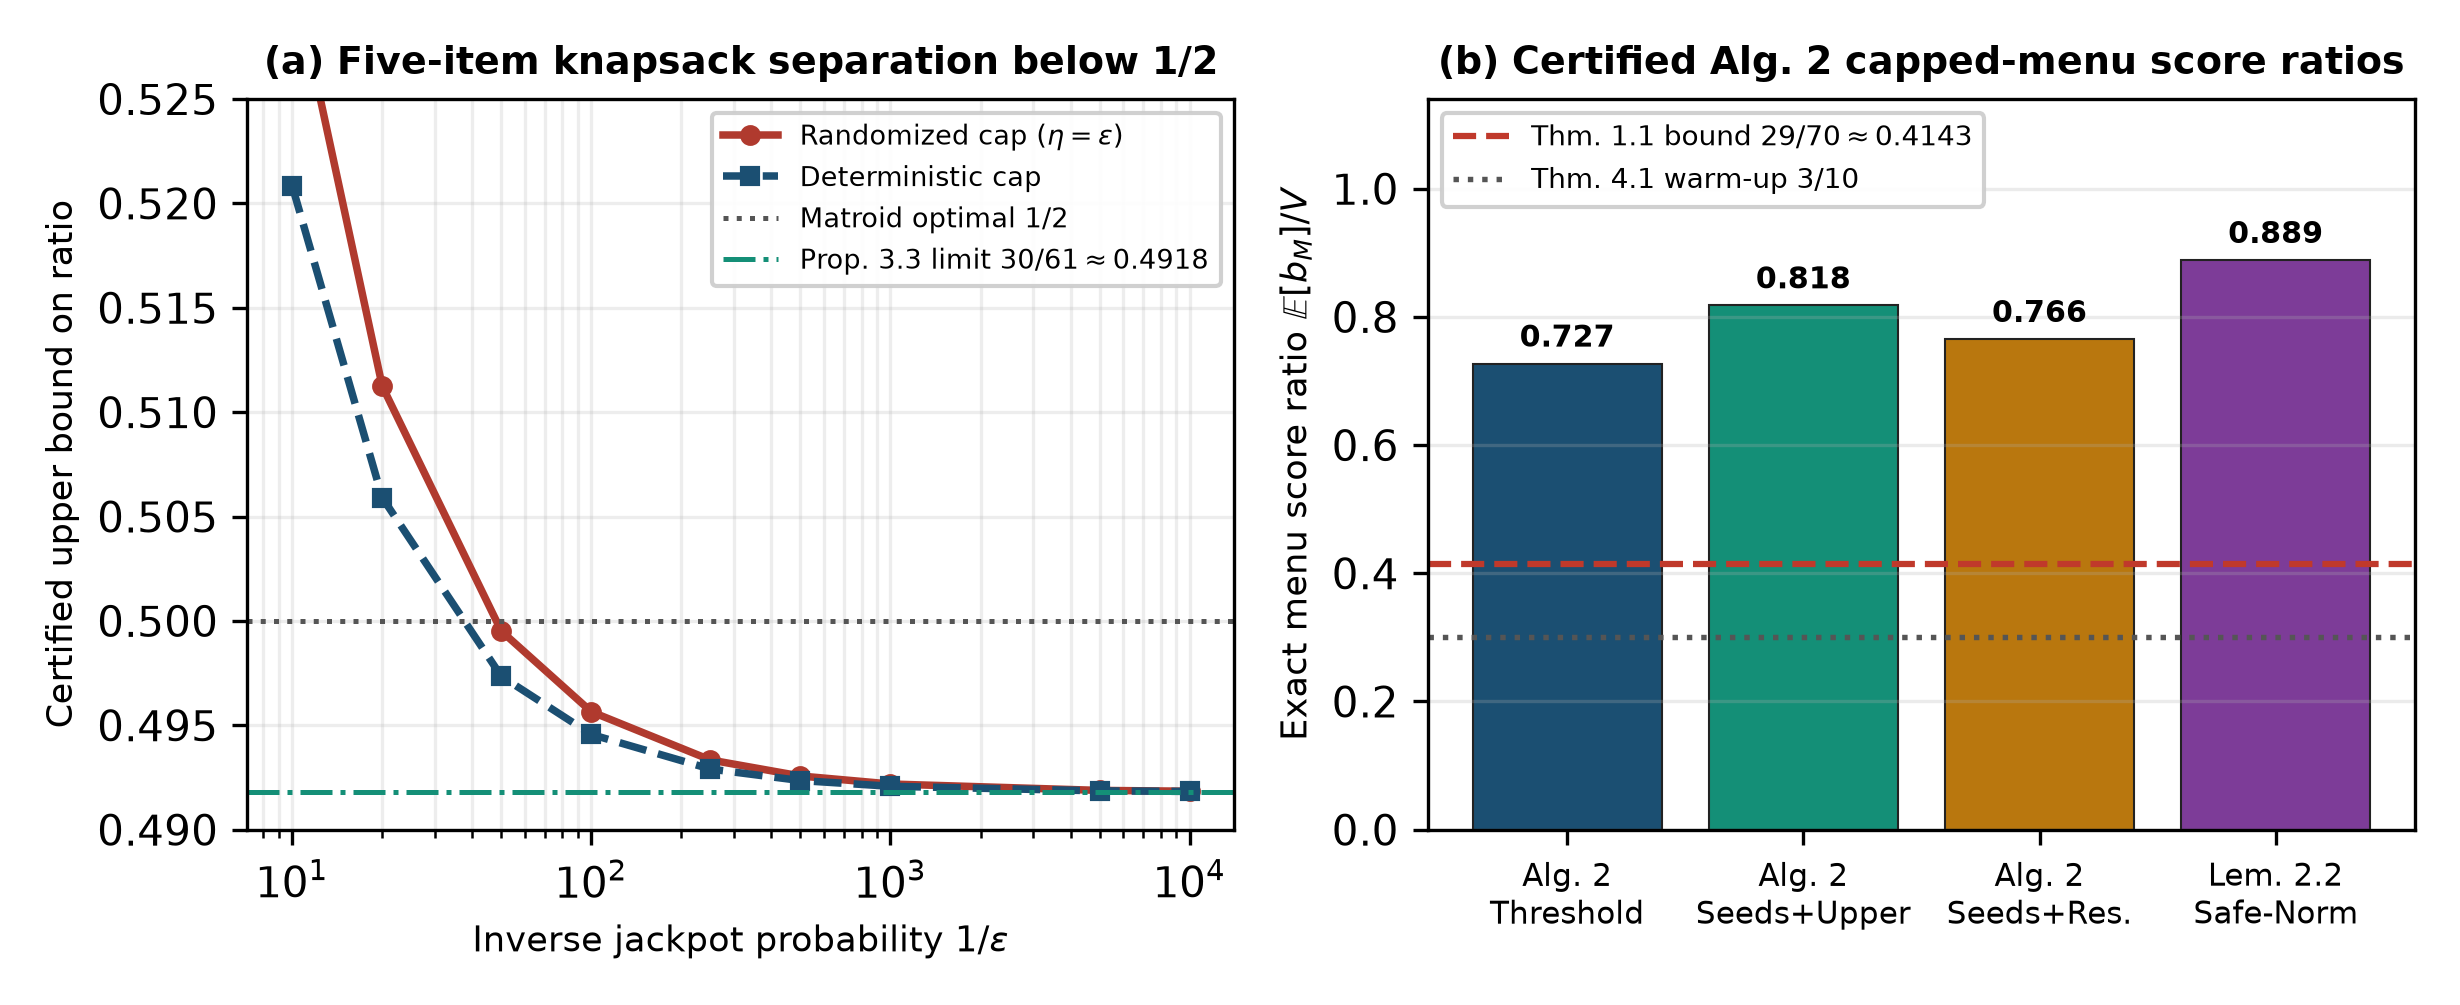
\includegraphics[width=\columnwidth]{../figures/fig1_knapsack_and_menus.png}
  \caption{(a) Exact deterministic and randomized five-item knapsack upper bounds converging below $1/2$ to $30/61 \approx 0.4918$ as $\varepsilon = \eta \downarrow 0$. (b) Exact Algorithm~2 capped-menu score ratios across all four Mode~3 instances, all strictly exceeding $29/70$.}
  \label{fig:knap}
\end{figure}

\paragraph{Five-Item Knapsack \& Algorithm~2 Scores (Fig.~\ref{fig:knap}).}
Mode~1 ($0.333$--$0.443\,\mathrm{ms}$) reproduces $V = 1011/50$, deterministic ratio $500/1011$, and randomized ratio $5011/10110$ at $\varepsilon = \eta = 1/100$, plus tighter sequences approaching $30/61$ at $\varepsilon = 1/10000$ ($16667037/33887000 \approx 0.49184$). Mode~3 ($0.276$--$2.611\,\mathrm{ms}$) certifies all three Algorithm~2 body types and Lemma~2.2 normalization with exact ratios $8/11$, $9/11$, $49/64$, and $8/9$, all strictly exceeding $29/70$.

\begin{figure}[t]
  \centering
  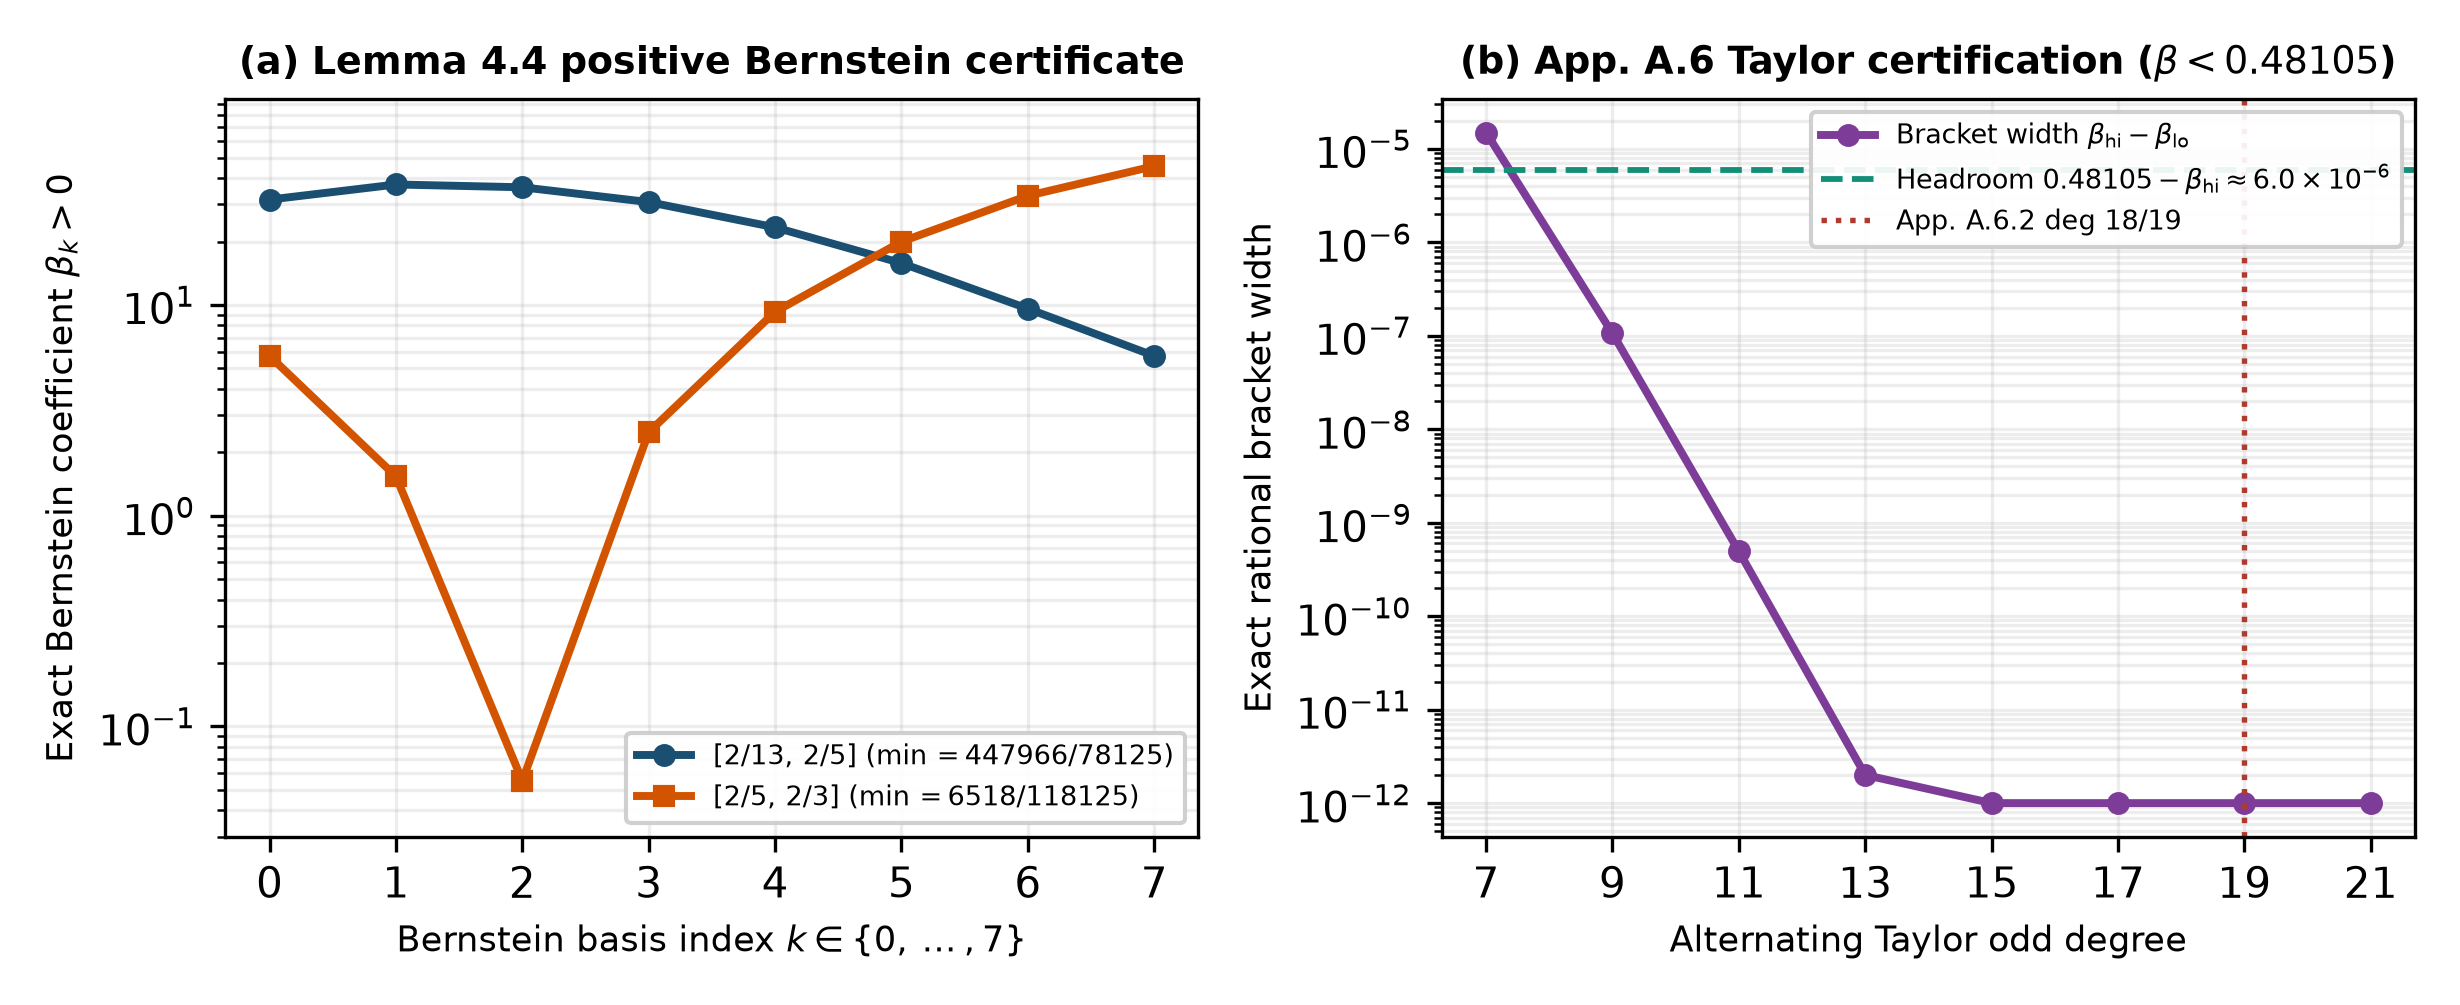
\includegraphics[width=\columnwidth]{../figures/fig2_bernstein_and_taylor_beta.png}
  \caption{(a) All 8 exact positive degree-7 Bernstein coefficients of $P(b)$ on $[2/13, 2/5]$ and $[2/5, 2/3]$, reproducing Abdi et al.'s exact minima $447966/78125$ and $6518/118125$. (b) Exact alternating-Taylor bracket width $\beta_{\mathrm{hi}} - \beta_{\mathrm{lo}}$ across odd degrees $7$--$21$, certifying $\beta \le 0.481043999746 < 0.48105$.}
  \label{fig:bern}
\end{figure}

\paragraph{Bernstein $3/10$ \& Appendix~A $\beta < 0.48105$ (Fig.~\ref{fig:bern}).}
Mode~2 ($0.603$--$0.877\,\mathrm{ms}$) reproduces Abdi et al.'s exact Bernstein minima $447966/78125$ on $[2/13, 2/5]$ and $6518/118125$ on $[2/5, 2/3]$, plus two refined subintervals ($[2/13, 1/4]$ and $[1/2, 2/3]$). Mode~4 ($0.185$--$0.249\,\mathrm{ms}$) certifies exact alternating-Taylor brackets across odd degrees $11, 15, 19, 21$; at Abdi et al.'s canonical degree $18/19$, the exact rational interval $[0.481043999745, 0.481043999746]$ matches~\cite[Sec.~A.6.1]{abdi2026downward} to all 12 decimal places.

\begin{figure}[t]
  \centering
  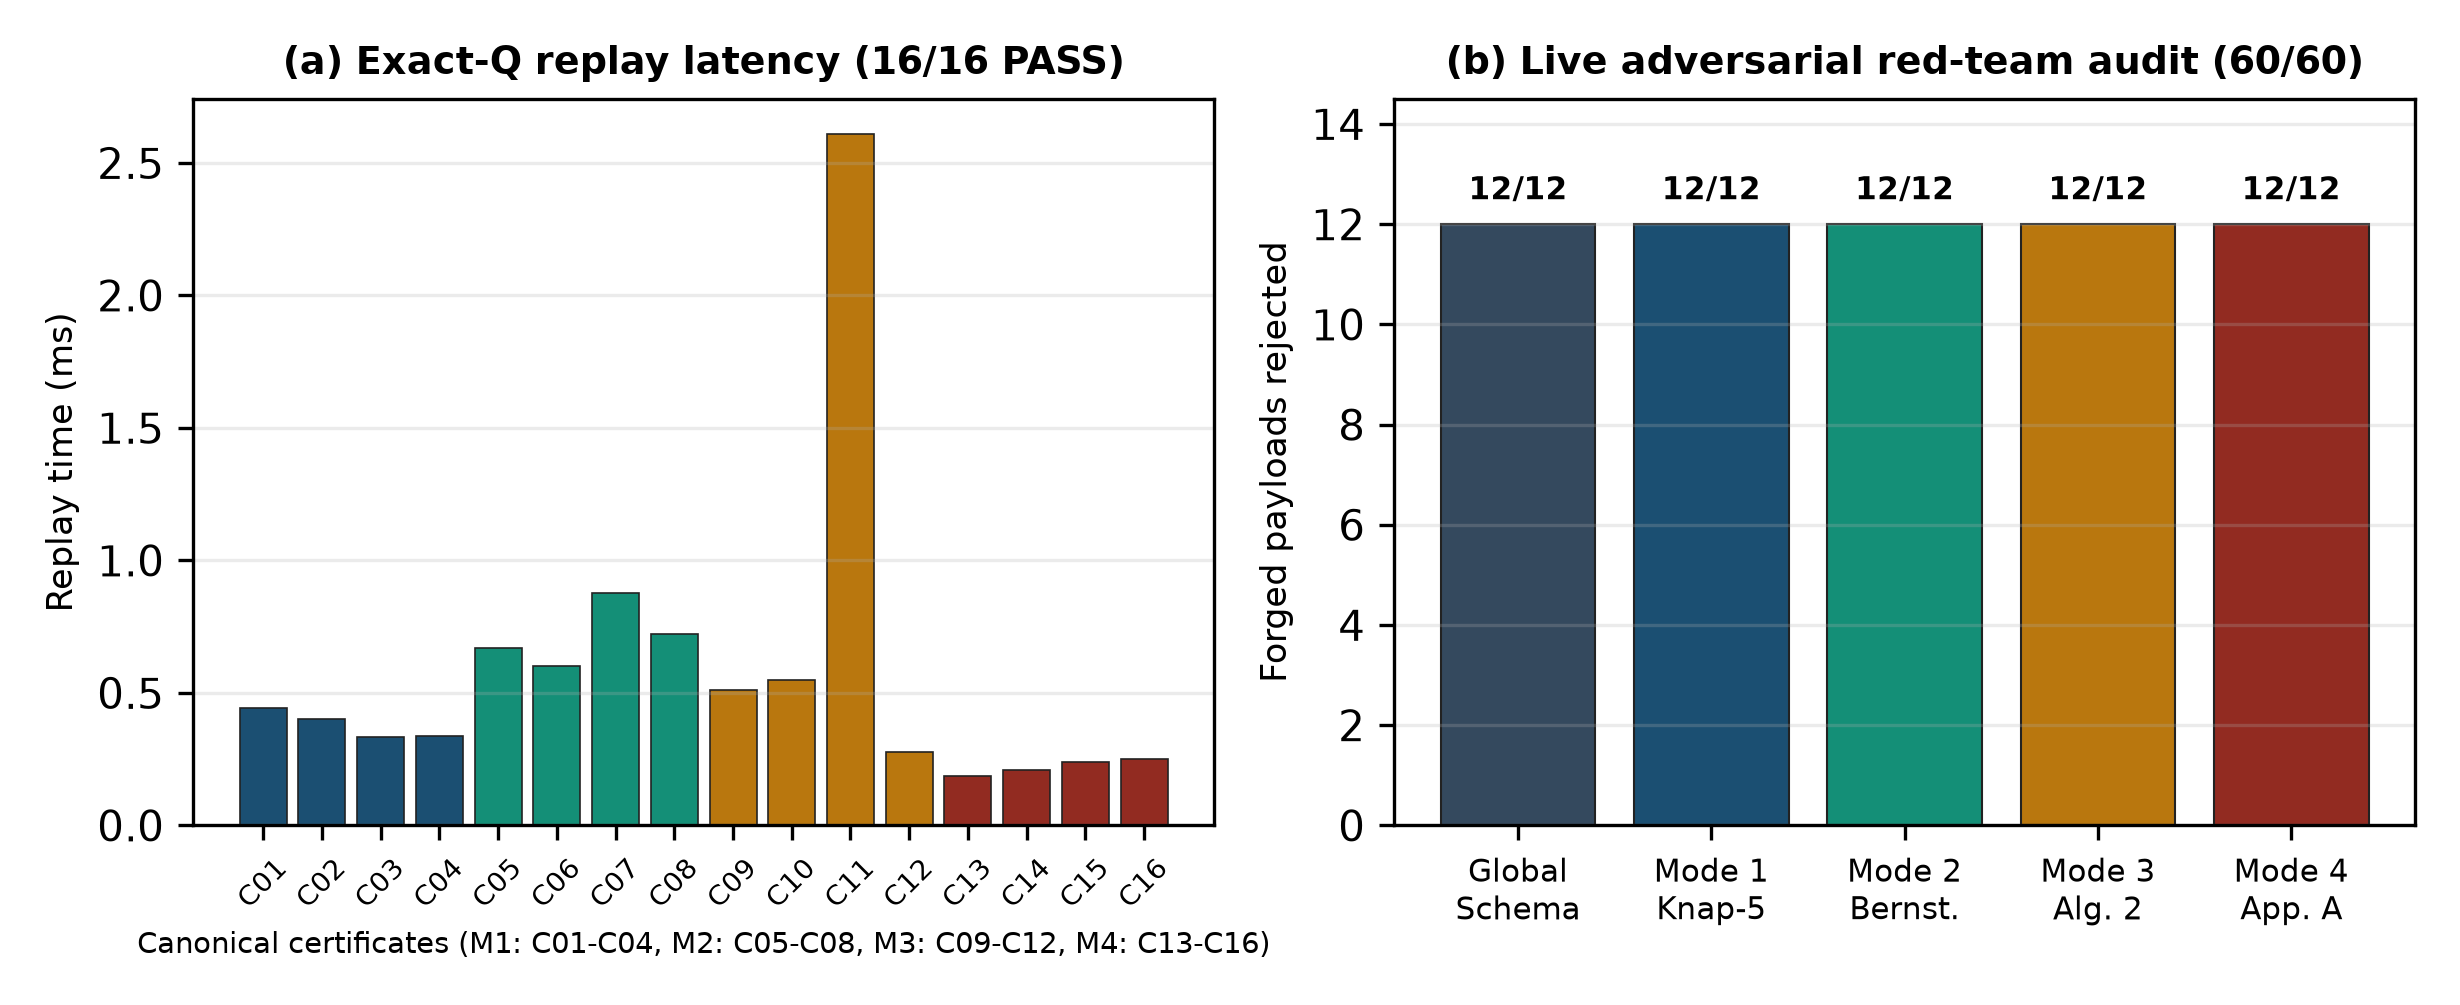
\includegraphics[width=\columnwidth]{../figures/fig3_certificate_replay_atlas.png}
  \caption{(a) Exact zero-float replay latency ($0.185$--$2.611\,\mathrm{ms}$) across all 16 canonical \texttt{DC-DELEG-CERT-1.0} certificates. (b) Live adversarial red-team audit rejecting 60/60 forged payloads across all five categories.}
  \label{fig:atlas}
\end{figure}

\paragraph{Replay Latency and 60/60 Red-Team Audit (Fig.~\ref{fig:atlas}).}
All 16 canonical certificates replay in $0.185$--$2.611\,\mathrm{ms}$ (total $9.21\,\mathrm{ms}$). The live adversarial suite (\texttt{tests/test\_suite.py}) tests 60 targeted forgeries---12 global schema/type/rational/newline/\texttt{"-0"}/depth attacks plus 12 domain attacks per mode (broken knapsack means, negative Bernstein coefficients on unsplit $[2/13, 2/3]$, non-downward-closed families, broken Lemma~2.2 safe singletons, invalid Taylor parity, and false $\beta$ bounds)---achieving \textbf{60/60 (100\%)} rejection.

\section{Conclusion}\label{sec:conc}
We delivered a self-contained, zero-floating-point verification framework for Abdi et al.'s downward-closed delegation bounds~\cite{abdi2026downward}, combining 18 zero-\texttt{sorry}, zero-\texttt{Classical.choice} Lean~4.35.0 theorems with the exact-$\QQ$ verifier \texttt{DC-DELEG-CERT-1.0}, 16 canonical certificates, and 60/60 live adversarial forgery rejections.

\bibliographystyle{plain}
\bibliography{references}
\end{document}
